% =====================================================================
% Rapport : Détection d'objets avec YOLO (sujet A)
% Template basé sur le « Guide du contenu de rapport » et sur la survey
% Zou et al., « Object Detection in 20 Years: A Survey » (arXiv:1905.05055)
% Compilation : pdflatex + bibtex + pdflatex x2  (ou Overleaf, par défaut)
% Les zones \todo{...} sont à remplacer par VOS résultats et VOS mots.
% =====================================================================
\documentclass[11pt,a4paper]{article}

\usepackage[utf8]{inputenc}
\usepackage[T1]{fontenc}
\usepackage[french]{babel}
\usepackage[margin=2.3cm]{geometry}
\usepackage{graphicx}
\usepackage{booktabs}
\usepackage{array}
\usepackage{amsmath,amssymb}
\usepackage{xcolor}
\usepackage{caption}
\usepackage{listings}
\usepackage{float}
\usepackage[numbers,sort&compress]{natbib}
\usepackage[colorlinks=true,linkcolor=blue!50!black,citecolor=blue!50!black,urlcolor=blue!50!black]{hyperref}

\captionsetup{font=small,labelfont=bf}
\setlength{\parskip}{0.4em}
\setlength{\parindent}{0pt}
\graphicspath{{figures/}}

% Zones à remplir : visibles en rouge, faciles à retrouver
\newcommand{\todo}[1]{\textcolor{red}{[#1]}}

% Style pour les commandes
\lstset{basicstyle=\ttfamily\footnotesize,breaklines=true,frame=single,
        columns=fullflexible,keepspaces=true}

% ---------------------------------------------------------------------
\title{Détection et localisation d’objets avec le modèle YOLO}
\author{RAKOTOARIMANANA Joy Sandra Hasina \and ANDRIAMIRINDRAMANANA Harifaly Lunard
\\[0.3cm]
    \small Parcours MAFI \& Calcul Numérique}

\date{}

\begin{document}
\maketitle

% =====================================================================
% 1. RÉSUMÉ (5 à 8 lignes) : problème -> méthode -> résultat -> conclusion
% =====================================================================

\tableofcontents
\newpage

% =====================================================================
% 2. INTRODUCTION (~1 page, 5 paragraphes)
% =====================================================================
\section{Introduction}


La détection d’objets est une tâche de vision par ordinateur qui permet de reconnaître et de localiser des objets dans des images ou des vidéos pour des applications comme la conduite autonome, la surveillance et l’imagerie médicale. Les premières méthodes de détection d’objets, comme le détecteur de Viola-Jones et l’histogramme des gradients orientés (HOG) associé aux machines à vecteurs de support (SVM), reposaient sur des caractéristiques conçues manuellement et des fenêtres glissantes. Ces méthodes peinaient souvent à détecter avec précision les objets dans les scènes complexes contenant plusieurs objets de formes et de tailles variées.\\[0.1cm]
Parmi les diverses méthodes dévelopées pour cette tâche, l'algorithme YOLO( You Only Look Once) s'est distingué par sa capacité à réaliser des détections en temps réel avec une precision remarquable.\\[0.1cm]
Ce projet se propose d'explorer les fondements de l'algorithme YOLO et d'examiner son foncionnement, ses avantages et ses applications pratiques.\\[0.1cm]
A travers ce rapport , nous visons à fournir une compréhension approfondie des principes de fonctionnement de YOLO, à analyser les performances du modèle et à illustrer des cas d'utilisation concrets qui démontrent le potentiel de cette technologie dans divers contextes.

\section{Rappel}
\subsection{Les Réseaux de Neurones Convolutifs(CNN)}
Contrairement aux réseaux de neurones classiques(MLP) qui traitent les entrées comme des vecteurs plats, les CNN sont conçus pour traiter des données ayant une structure de grille, comme les images.
Les composants clés d'un CNN incluent:
\begin{enumerate}
    \item \textbf{Couches de Convolution}: elles appliquent des filtres (kernels) sur l'image pour extraire des caractéristiques visuelles(bords,textures,formes)
    \item \textbf{Fonction d'activation }(ReLU): elles introduisent de la non-linéarité dans le réseau, permettant d'apprendre des motifs complexes.
    \item \textbf{Pooling} (Mise en commun): cette opération réduit la dimensionnalité des cartes de caractéristiques, rendant le modèle plus léger et moins sensible aux petites translations de l'image
\end{enumerate}

Les réseaux neuronaux convolutifs basés sur des régions (R-CNN) ont changé notre approche de la détection d’objets. Ils représentent une étape importante dans l’histoire de la vision par ordinateur. Pour comprendre comment des modèles comme Ultralytics YOLOv8 ont vu le jour, nous devons d’abord comprendre des modèles comme R-CNN.

\section{R-CNN}

Créée par Ross Girshick et son équipe, l’architecture du modèle R-CNN génère des propositions de régions, extrait des caractéristiques à l’aide d’un réseau neuronal convolutif (CNN) préentraîné, classe les objets et affine les boîtes englobantes.

\subsection{Fonctionnalité de R-CNN}
\begin{figure}[htbp]
    \centering
    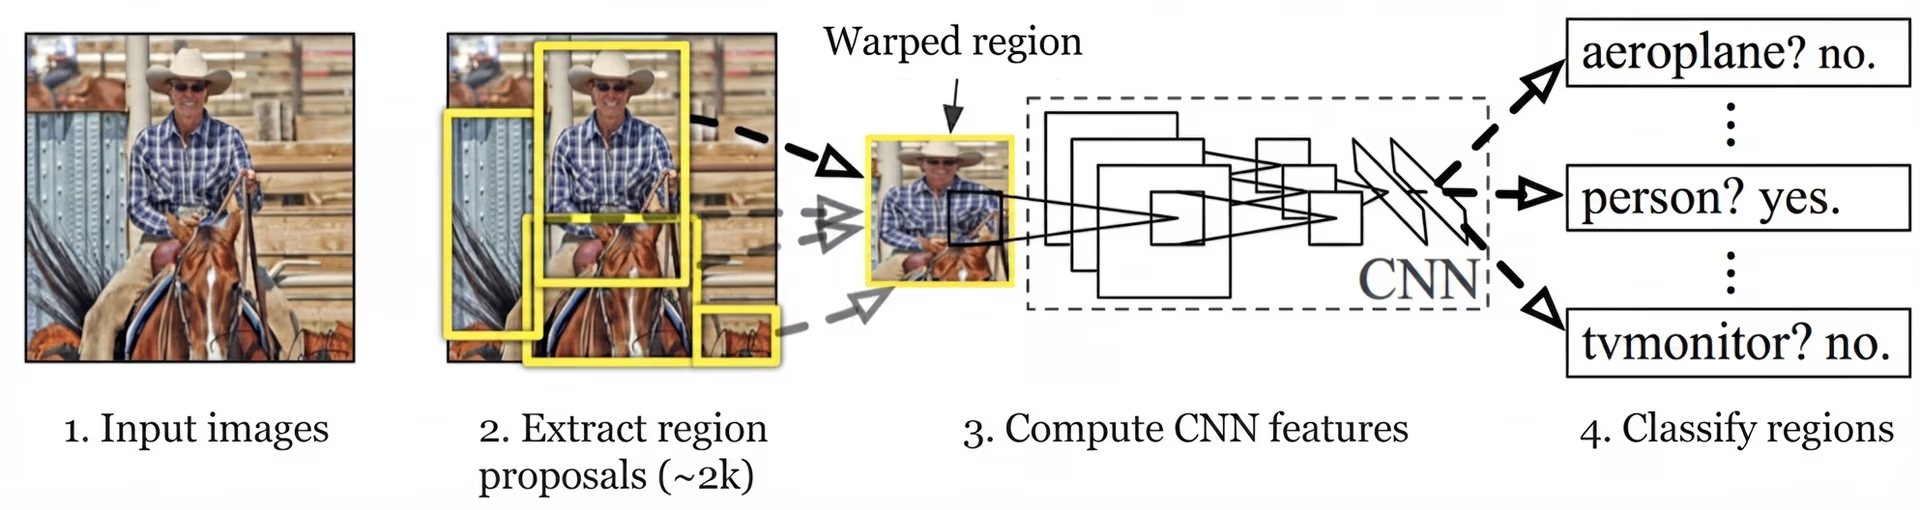
\includegraphics[width=0.6\textwidth]{important.png}
    \caption{Fonctionnement de R-CNN}
    \label{fig:mon-etiquette}
\end{figure}
Le processus de détection d’objets du modèle R-CNN comprend trois étapes principales:
\begin{enumerate}
    \item générer des propositions de régions,
    \item extraire des caractéristiques 
    \item classer les objets tout en affinant leurs boîtes englobantes
\end{enumerate}

Décortiquons chaque étape maintenant pour bien comprendre son fonctionnement



\subsection{Proposition de régions}
Lors de la première étape, le modèle R-CNN parcourt l’image pour créer de nombreuses propositions de régions. Ces propositions correspondent à des zones susceptibles de contenir des objets. Des méthodes comme Selective Search examinent différents aspects de l’image, tels que la couleur, la texture et la forme, puis la divisent en plusieurs parties. Selective Search commence par découper l’image en petites parties, puis fusionne les parties similaires pour former des zones d’intérêt plus grandes. Le processus se poursuit jusqu’à la génération d’environ 2 000 propositions de régions.

\begin{figure}[htbp]
    \centering
    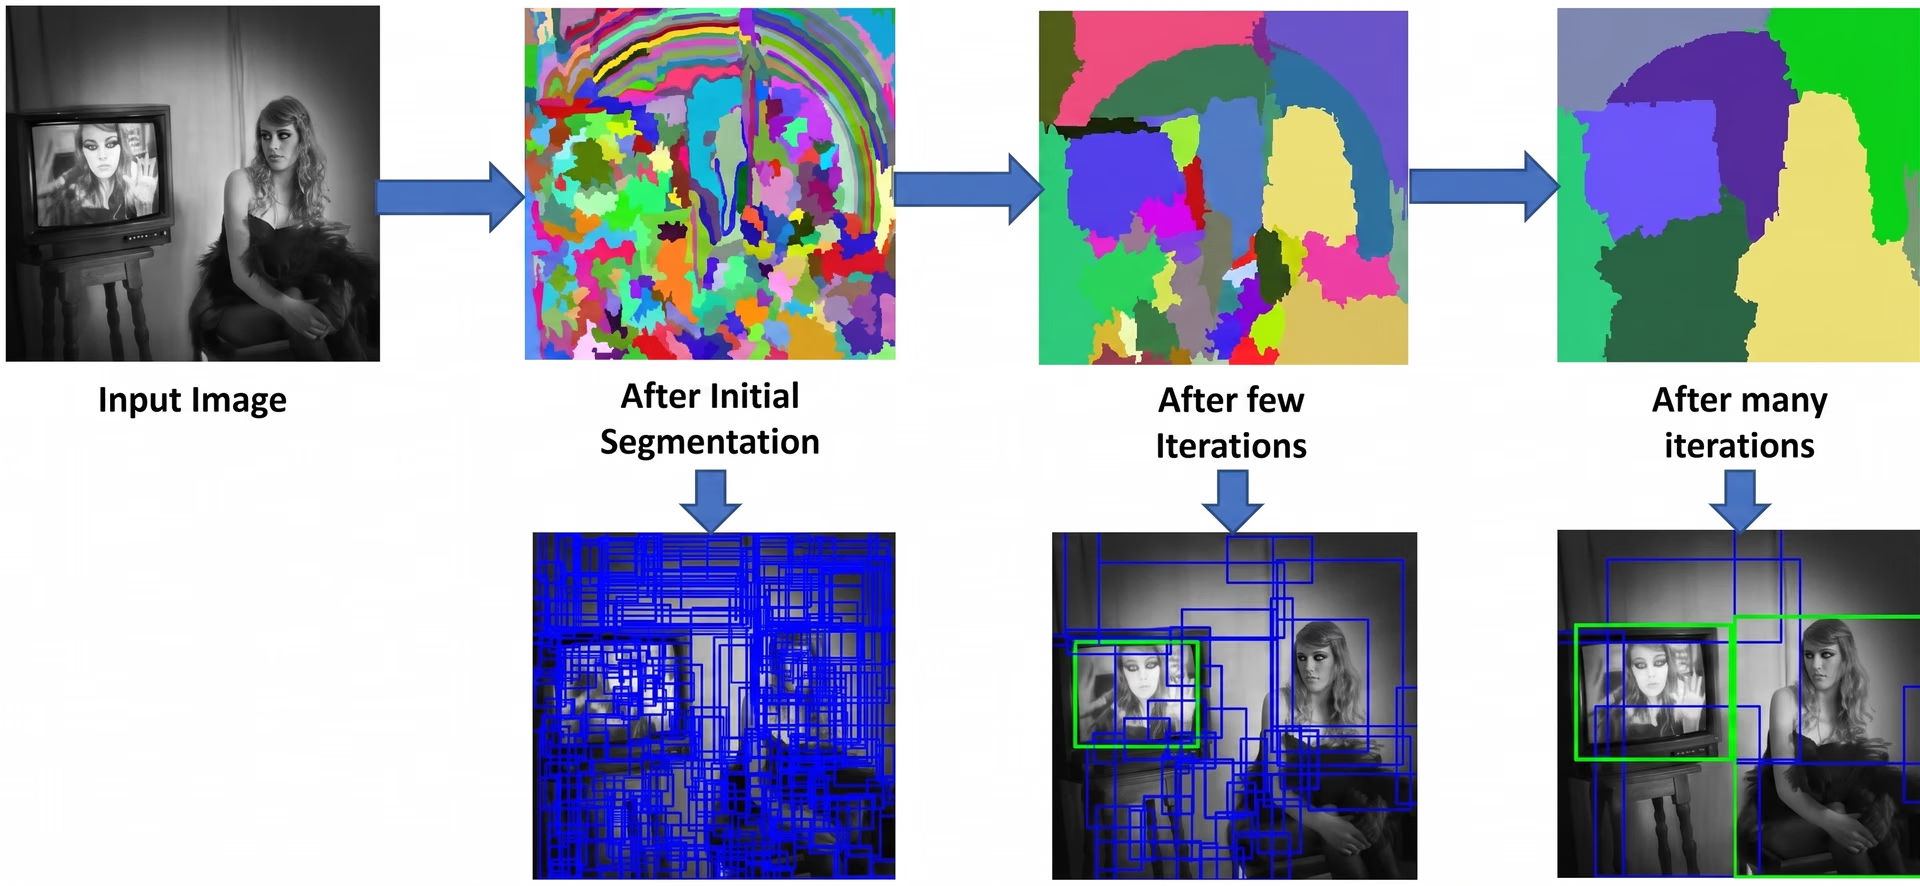
\includegraphics[width=0.8\textwidth]{RCNN.png}
    \caption{Fonctionnement de Selective Search}
    \label{fig:mon-etiquette}
\end{figure}
Ces propositions de régions permettent d’identifier tous les endroits possibles où un objet pourrait se trouver. Lors des étapes suivantes, le modèle peut traiter efficacement les zones les plus pertinentes en se concentrant sur ces régions spécifiques plutôt que sur l’image entière.

\subsection{Extraction des caractéristiques de l'image}
L’étape suivante du processus de détection d’objets du modèle R-CNN consiste\textbf{ à extraire des caractéristiques des propositions de régions}. Chaque proposition est redimensionnée à une taille uniforme attendue par le CNN (par exemple, 224x224 pixels). \textbf{Le redimensionnement aide le CNN à traiter efficacement chaque proposition}.\\[0.1cm]
Avant la déformation, chaque proposition de région est légèrement agrandie pour inclure 16 pixels de contexte supplémentaire autour de la région et fournir davantage d’informations environnantes pour une meilleure extraction des caractéristiques.\\[0.1cm]
\textbf{Une fois redimensionnées, ces propositions de régions sont transmises à un CNN} comme AlexNet, généralement préentraîné sur un grand jeu de données comme ImageNet.\textbf{ Le CNN traite chaque région pour en extraire des vecteurs de caractéristiques} de grande dimension qui capturent des détails importants tels que \textbf{les contours, les textures et les motifs}\\[0.1cm]
Ces vecteurs de caractéristiques condensent les informations essentielles des régions. Ils transforment les données brutes de l’image en un format que le modèle peut utiliser pour une analyse plus poussée.

\begin{figure}[htbp]
    \centering
    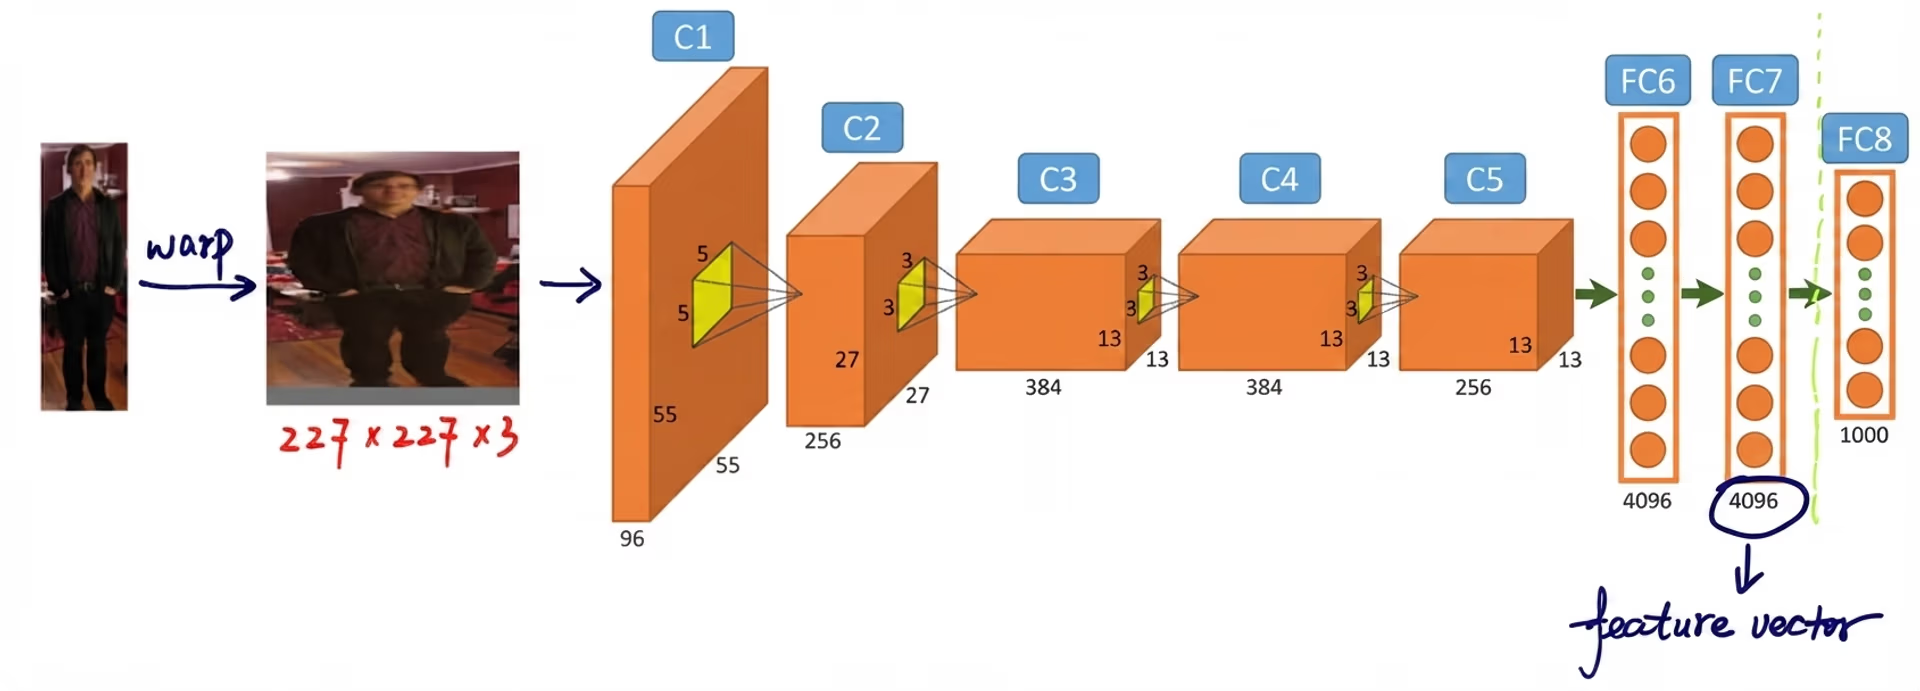
\includegraphics[width=0.8\textwidth]{Extraction.png}
    \caption{Extraire les caractéristiques d’une proposition de région à l’aide d’AlexNet.}
    \label{fig:mon-etiquette}
\end{figure}
\subsection{Classification des objets}
La troisième étape consiste à classer les objets dans ces régions. Il s’agit de déterminer la catégorie ou la classe de chaque objet repéré dans les propositions. Les vecteurs de caractéristiques extraits sont ensuite transmis à un classificateur d’apprentissage automatique.\\[0.1cm]

Dans R-CNN, les machines à vecteurs de support (SVM) sont couramment utilisées à cette fin. Chaque SVM est entraînée à reconnaître une classe d’objet précise en analysant les vecteurs de caractéristiques et en déterminant si une région donnée contient une instance de cette classe.\\[0.1cm]
En pratique, chaque catégorie d’objets dispose d’un classificateur dédié qui vérifie la présence de l’objet correspondant dans chaque proposition de région.\\[0.1cm]
Pendant l’entraînement, les classificateurs reçoivent des données étiquetées comportant des échantillons positifs et négatifs :
\begin{enumerate}
    \item Échantillons positifs : régions contenant l’objet cible.
    \item Échantillons négatifs : régions ne contenant pas l’objet
\end{enumerate}
Les classificateurs apprennent à distinguer ces échantillons. La régression des boîtes englobantes affine davantage la position et la taille des objets détectés en ajustant les boîtes initialement proposées pour mieux correspondre aux contours réels des objets. En combinant la classification et la régression des boîtes englobantes, le modèle R-CNN peut identifier et localiser précisément les objets.
\subsection{Affiner les détections avec NMS}
Après les étapes de classification et de régression des boîtes englobantes, le modèle génère souvent plusieurs boîtes englobantes qui se chevauchent pour un même objet. La suppression non maximale (NMS) est appliquée pour affiner ces détections en conservant les boîtes les plus précises.\\[0.1cm]
Le modèle élimine les boîtes redondantes et chevauchantes en appliquant la NMS et ne conserve que les détections les plus fiables.\\[0.2cm]
NMS évalue les scores de confiance de toutes les boîtes englobantes (qui indiquent la probabilité qu’un objet détecté soit effectivement présent) et supprime celles qui chevauchent fortement des boîtes ayant obtenu un score plus élevé.

\begin{figure}[htbp]
    \centering
    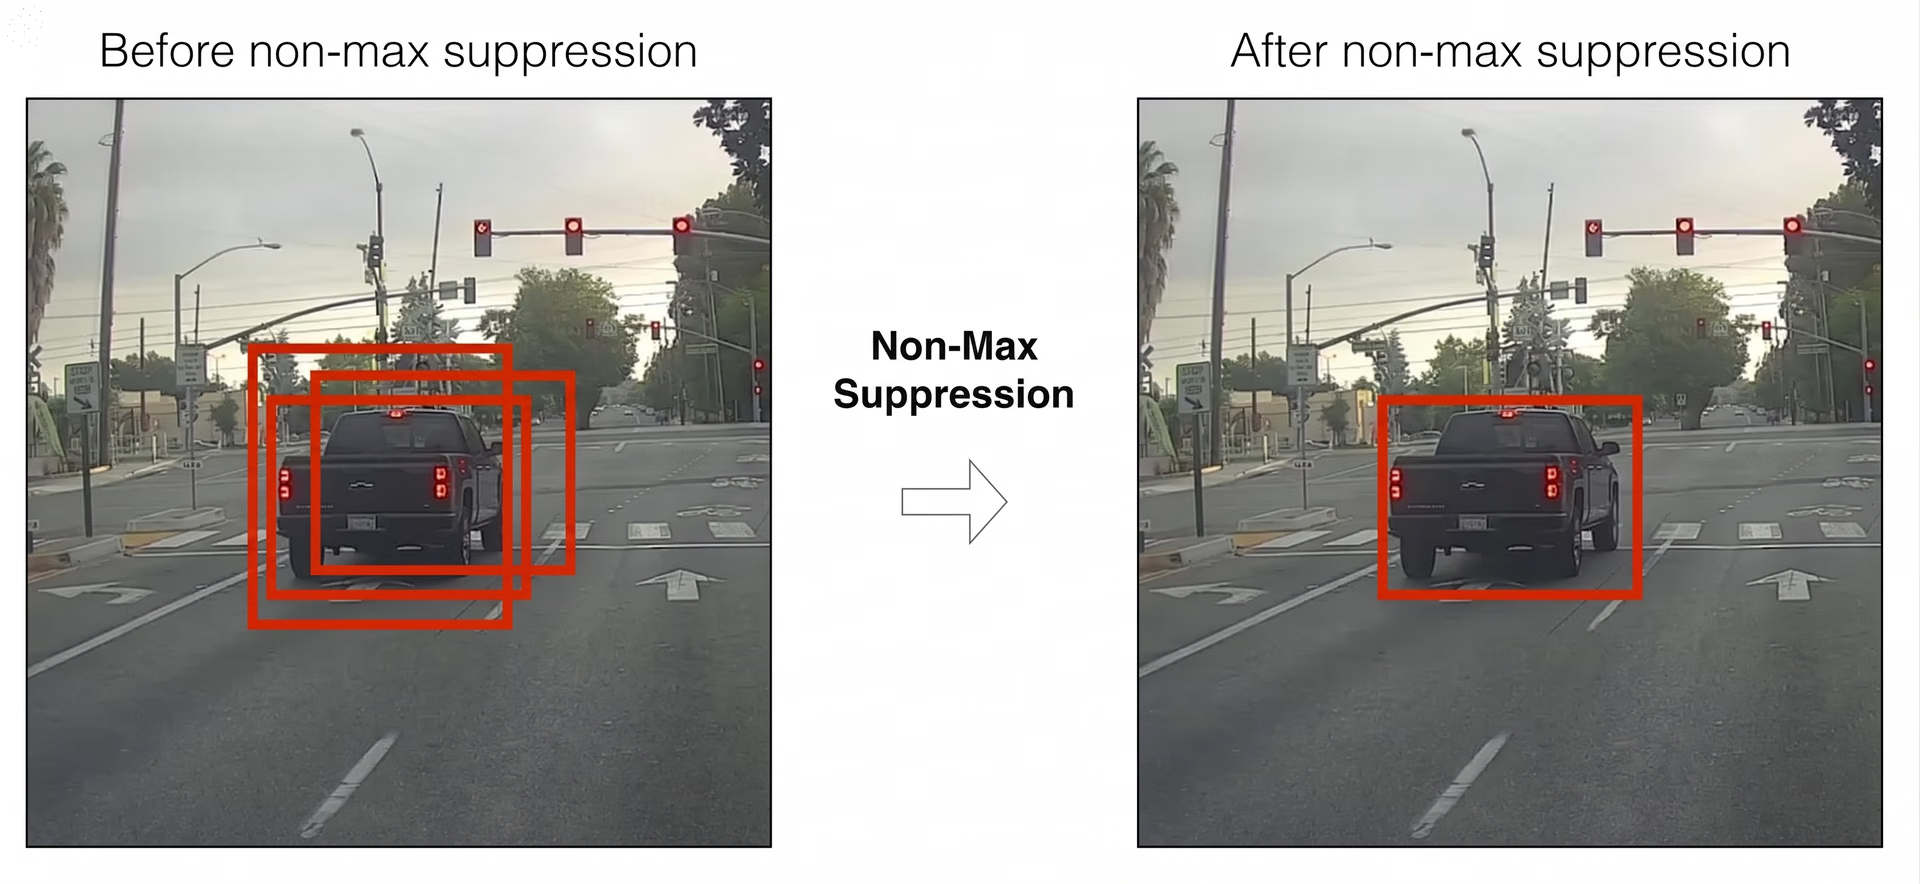
\includegraphics[width=0.7\textwidth]{NMS.png}
    \caption{ Exemple de suppression non maximale}
    \label{fig:mon-etiquette}
\end{figure}
R-CNN a ouvert la voie à des modèles comme Fast R-CNN, Faster R-CNN qui ont encore amélioré l’efficacité et la précision.
\section{YOLO- You Only Look Once}
\subsection{Définition}
\textbf{YOLO} est un algorithme de détection d'objets en temps réel qui révolutionne le domaine de la vision par ordinateur. Contrairement aux méthodes traditionnelles qui nécessitent plusieurs passes pour détecter des objets dans une image, YOLO effectue cette tâche en une seule passe à travers un réseau neuronal convolutif (CNN) (le réseau ne regarde l'image qu'une seule fois pour tout prédire)
% Packages nécessaires dans le préambule :
% \usepackage[french]{babel}   % pour obtenir « Tableau 1 »
% \usepackage{array}

\begin{table}[htbp]
\centering
\renewcommand{\arraystretch}{1.4}
\begin{tabular}{|>{\bfseries}p{5cm}|p{9cm}|}
\hline
\textbf{Caractéristiques} & \textbf{Description} \\
\hline
Nom & YOLO (You Look Only Once). \\
\hline
Créateurs & Joseph Redmon et Ali Farhadi (2015). \\
\hline
Type & Algorithme de détection d'objets en temps réel basé sur des réseaux de neurones convolutifs (CNN). \\
\hline
Versions & De YOLOv1 à YOLOv9. \\
\hline
Applications & Utilisé dans les véhicules autonomes, la vidéosurveillance et la robotique \dots \\
\hline
Métriques de performance & Utilise l'intersection over Union (IoU) pour évaluer la précision des prédictions de boîtes englobantes. \\
\hline
\end{tabular}
\caption{Caractéristiques de YOLO.}
\end{table}

\subsection{YOLO :Comment ça marche ?}
Cette partie décrit l’architecture de YOLO.\\[0.2cm]
\textbf{Séparation en grille}\\[0.2cm]
Le principe de base de YOLO est de diviser l’image en plus petites parties à l’aide d’une grille de dimension $S \times S$

\begin{figure}[H]
    \centering
    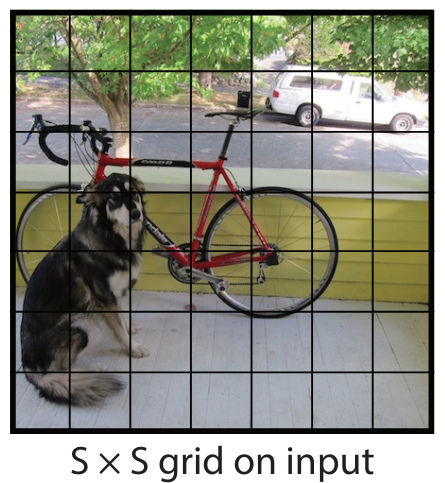
\includegraphics[width=0.4\textwidth]{SS.png}
    \caption{Séparation en grille}
    \label{fig:mon-etiquette}
\end{figure}
La cellule contenant le centre d’un objet (par exemple un chien ou un vélo) est responsable de sa détection (pour le calcul du loss). Chaque cellule de la grille prédit $B$ bounding boxes(paramétrable) et un score de confiance pour chacune.\\[0.1cm]
La "bounding box" prédite contient les 5 valeurs $x,y,h,w,\text{et confiance}$ où $(x,y)$ est la position du centre dans la grille, $(w,h)$ la largeur et la hauteur sont prédites par rapport à l’image entière, et enfin la prédiction de confiance représente l'IoU entre la boîte prédite(predicted box) et toute boîte de vérité terrain(any ground truth box). 
\\[0.1cm]
Pour calculer la précision de notre bounding box lors de l’entraînement (composante du loss), on utilise l’intersection over union, définie comme:
$$\frac{pred_{box} \cap label_{box}}{pred_{box} \cup label_{box}}$$
\begin{figure}[H]
    \centering
    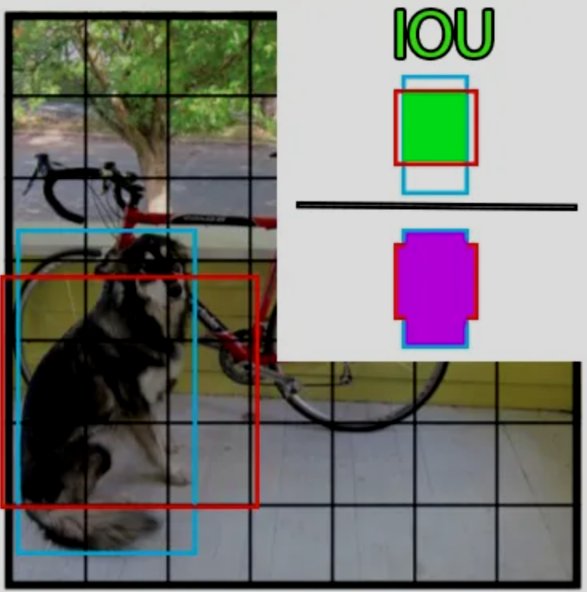
\includegraphics[width=0.4\textwidth]{IOU.png}
    \caption{Séparation en grille}
    \label{fig:mon-etiquette}
\end{figure}
En plus de prédire la bounding box et la confiance, chaque cellule prédit aussi la classe de l’objet. Cette classe est représentée par un vecteur $\text{one\_hot}$ (qui contient uniquement des 0 sauf un 1 dans la bonne classe) dans les annotations.\\[0.1cm]
Il est important de noter que chaque cellule peut prédire plusieurs bounding boxes mais une seule classe.\\[0.1cm]
Chaque cellule de la grille prédit également probabilités de classe conditionnelles, $Pr(Classe_i | Objet)$. Ces probabilités sont conditionnées par le fait que la cellule de la grille contienne un objet.Nous ne prédisons qu’un seul ensemble de probabilités de classe par cellule de la grille, quel que soit le nombre de boîtes B.\\[0.1cm]

Maintenant qu’on a toutes les informations, on peut calculer la dimension de sortie du réseau. On a $S \times S$ cellules, chaque cellule prédit $B$ bounding boxes, confiance pour ces boîtes et  $C$ "class probabilities" (avec 
 le nombre de classes).
La prédiction du modèle est donc de taille : 
$$S \times S \times (C+B \times 5)$$
\begin{figure}[H]
    \centering
    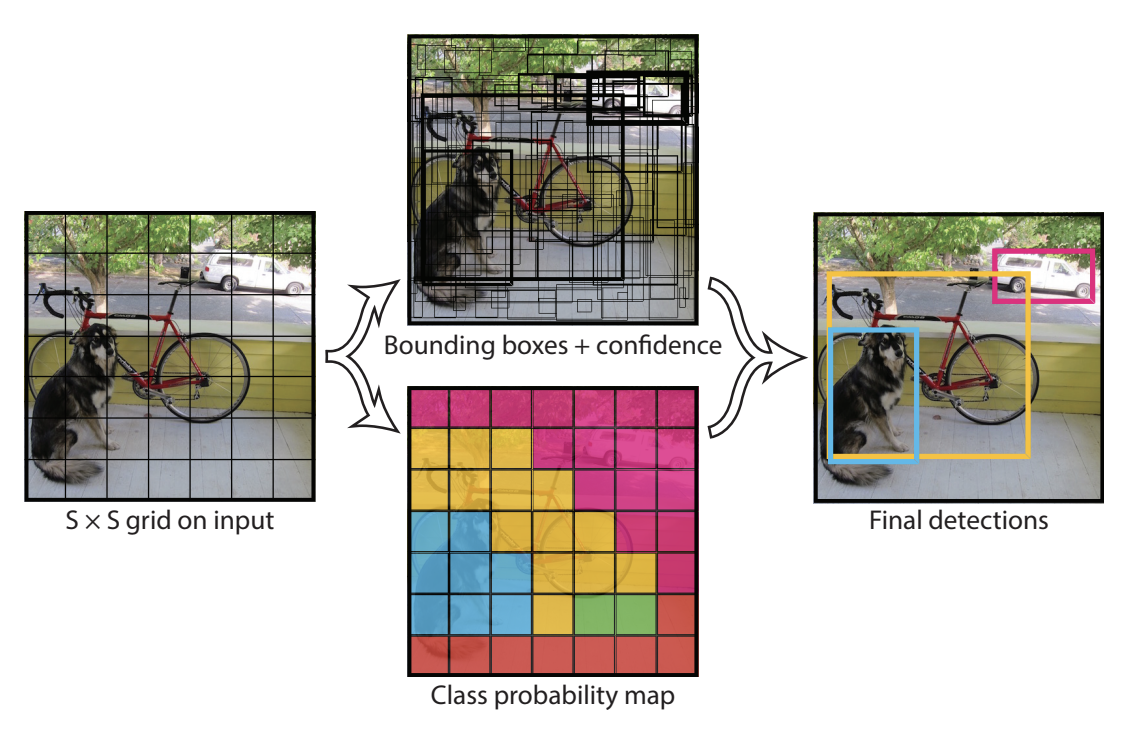
\includegraphics[width=0.8\textwidth]{yolo.png}
    \caption{Résultat final}
    \label{fig:mon-etiquette}
\end{figure}
La figure du centre en haut montre les bounding boxes prédites par le modèle (celles avec un trait plus épais ont des scores de confiance élevés).La figure du centre en bas montre la classe prédite dans chaque cellule (en bleu la classe chien, en jaune la classe vélo et en rose la classe voiture).\\[0.2cm]
Exemple : Pour évaluer YOLO sur Pascal VOC, on utilise $S=7$, $B=2$. Pascal VOC a 20 classes labelées donc $C=20$. Notre final prédiction est un $7 \times 7 \times 30$ tenseur.
\subsection{Architecture du modèle}
Elle comprend trois composants principaux : head, neck et backbone.
\begin{enumerate}
    \item \textbf{Backbone} : C’est la partie la plus importante du réseau, composée d’une série de convolutions pour détecter les features les plus importantes. Cette partie est souvent pré-entraînée sur un dataset de classification.
    \item \textbf{Neck} : a pour rôle d'extraire les caractéristiques pertinentes de l'ensemble des couches de la backbone, et de les combiner en caractéristiques utiles à notre tâche de détection
    \item \textbf{Head}: est responsable de la décision finale du reseau
\end{enumerate}
Les premières couches convolutionnelles du réseau extraient les caractéristiques de l'image tandis que les couches entièrement connectées prédisent les probabilités et les coordonnées de sortie.\\[0.1cm]

Notre architecture de réseau s'inspire du modèle GoogLeNet de classification d'images.Notre réseau comporte\textbf{ 24 couches de convolution}, suivies de \textbf{2 couches entièrement connectées}.
Au lieu des modules d'initialisation utilisés par GoogLeNet, nous employons simplement \textbf{des couches de réduction} $1 \times 1$, suivies de $3 \times 3$ \textbf{couches convolutives}. Le réseau complet est présenté dans la figure
\begin{figure}[H]
    \centering
    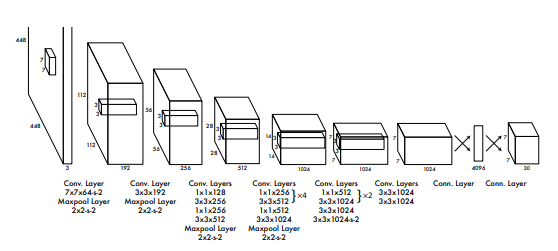
\includegraphics[width=1\textwidth]{Capture d’écran_2026-11-18_12-10-35.png}
    \caption{Architecture YOLO}
    \label{fig:mon-etiquette}
\end{figure}
\section{Principes de fonctionnement de YOLO}
Le fonctionnement de YOLO repose sur plusieurs étapes clés:
\begin{enumerate}
    \item \textbf{Division de l'image}: l'image d'entrée est divisée en une grille $S \times S$(système de grille ou grid system). Chaque cellule de la grille est responsable de la détection des objets dont le centre se trouve à l'intérieur de celle-ci
    \item \textbf{Prédiction des boîtes englobantes}: chaque cellule prédit $B$ boîtes englobantes et leurs scores de confiance. Ces boîtes sont définies par 5 paramètres : $x,y \quad (\text{position du centre}),w,h$(dimensions) et un score de confiance qui indique la probabilité qu'un objet soit présent
    \item  \textbf{Probabilités conditionnelles}: chaque cellule prédit également des probabilités conditionnelles pour chaque classe d'objet, permettant ainsi de déterminer à quelle classe appartient l'objet détecté
    \item \textbf{Filtrage et suppression des doublons}: pendant le test, YOLO applique un filtrage par seuil et une suppression non maximale (NMS) pour obtenir les résultats finaux, éliminant les prédictions redondantes
\end{enumerate}

% =====================================================================
% 5. MÉTHODES (2 pages)
% =====================================================================
\section{Métriques}
\begin{itemize}
  \item \textbf{IoU} : aire de l'intersection divisée par l'aire de l'union
        entre la boîte prédite et la boîte réelle. Une détection est correcte
        si l'IoU dépasse un seuil (par exemple 0{,}5).
  \item \textbf{Précision} : $\mathrm{TP}/(\mathrm{TP}+\mathrm{FP})$, part
        des détections correctes.
  \item \textbf{Rappel} : $\mathrm{TP}/(\mathrm{TP}+\mathrm{FN})$, part des
        objets réels retrouvés.
  \item \textbf{AP et mAP} : l'AP est l'aire sous la courbe
        précision-rappel d'une classe ; le mAP est la moyenne de l'AP sur les
        classes.
  \item \textbf{Vitesse} : temps d'inférence moyen par image, avec le
        matériel, la taille de lot et la résolution précisés.
\end{itemize}

\section{Amelioration de YOLO}
Nous avons vu que YOLO est un modèle très performant et rapide pour la détection d’objets dans les images. C’est pourquoi, de nombreux chercheurs ont cherché à l’améliorer en proposant diverses optimisations. Aujourd’hui encore, de nouvelles versions de YOLO sortent régulièrement.\\[0.2cm]
\textbf{YOLOv2 (2017)}: Introduction de l’idée d’ancres (anchors) pour améliorer la précision des prédictions de boîte. Passage de la résolution d’entrée de 224x224 à 416x416 pour améliorer la détection d’objets de petite taille.\\[0.1cm]
\textbf{YOLOv3 (2018)}: Utilisation d’un modèle plus profond avec une architecture Darknet-53, un réseau de neurones convolutifs résiduel. Détection multi-échelle, avec des prédictions faites à trois niveaux de granularité différents (feature maps de différentes tailles).\\[0.1cm]
\textbf{YOLOv4 (2020)}: Utilisation du backbone CSPDarknet53 pour une meilleure performance. Améliorations des têtes de détection avec PANet (Path Aggregation Network) pour améliorer les flux d’informations.Introduction du concept de Mosaic Data Augmentation pour enrichir la diversité des données d’entraînement. Ajout de diverses techniques modernes comme DropBlock, Mish activation, et SPP (Spatial Pyramid Pooling).\\[0.1cm]
\textbf{YOLOv5 (2020)} : Développé par Ultralytics. Pas de papier officiel, mais des améliorations pratiques dans l’implémentation et la performance. Modèle plus léger et plus facile à entraîner avec une meilleure gestion des dépendances.\\[0.1cm]
\textbf{YOLOv6 (2022)}: Nouveau backbone YOLOv6S, optimisé pour les performances en temps réel. Techniques avancées de réduction de la latence. Améliorations dans les méthodes d’augmentation des données et l’optimisation des hyperparamètres.\\[0.1cm]
\textbf{YOLOv7 (2022)}: Intégration de bag of freebies pour améliorer la précision sans augmenter le temps d’inférence. Architecture optimisée pour un compromis optimal entre vitesse et précision. Ajout de diverses techniques de régularisation pour améliorer la performance générale.\\[0.1cm]
\textbf{YOLOv8 (2023)}: Développé par Ultralytics. Encore plus optimisé pour les performances en temps réel et l’intégration mobile. Architecture flexible permettant des ajustements pour divers cas d’utilisation, y compris la détection, la segmentation et la classification\\[0.1cm]
\textbf{YOLO-World (2024)}: Utilisation d’un transformer encoder pour le texte permettant la détection open-vocabulary.






% =====================================================================
% 7. RÉSULTATS (2 pages) : présenter sans interpréter
% =====================================================================





\section{YOLOv8 : des principes de YOLOv1 aux variantes n et s}
\label{sec:yolov8}

\subsection{Des détecteurs à deux étages à YOLOv8}
Fast R-CNN \citep{girshick2015fast} calcule les caractéristiques de l'image
entière une seule fois, au lieu de repasser chaque région dans le réseau, ce
qui accélère nettement R-CNN. Faster R-CNN \citep{ren2015faster} remplace
ensuite Selective Search par un réseau qui génère lui-même les propositions
de régions. Ces méthodes restent des détecteurs à deux étages. YOLO
\citep{redmon2016yolo} propose au contraire de prédire directement les
boîtes et les classes en une seule passe.

\subsection{Architecture de YOLOv8}
La description de YOLO donnée plus haut correspond à YOLOv1. Le modèle
utilisé dans les expériences, YOLOv8 \citep{jocher2023ultralytics}, en
conserve l'idée d'une détection en une seule passe, mais son architecture
diffère : il n'utilise pas d'ancres (\emph{anchor-free}), sépare dans la
tête de détection les branches de classification et de régression des boîtes
(\emph{decoupled head}), s'appuie sur un backbone de type CSP à blocs C2f et
sur un neck de type PAN-FPN qui combine plusieurs échelles de cartes de
caractéristiques, ce qui est utile pour les objets de tailles variées.

\subsection{Variantes YOLOv8n et YOLOv8s}
Ultralytics propose plusieurs variantes de YOLOv8 qui partagent la même
architecture et diffèrent par la profondeur et la largeur du réseau. Deux
d'entre elles sont comparées ici : YOLOv8n (\emph{nano}, 3,13 M de
paramètres) et YOLOv8s (\emph{small}, 11,13 M de paramètres). La résolution
d'entrée est un hyperparamètre indépendant de la variante : l'augmenter ne
change pas le nombre de paramètres mais augmente le nombre d'opérations par
image. C'est cette distinction qui permet de comparer deux leviers : plus de
capacité (modèle plus grand) ou plus de détails (résolution plus élevée).

\subsection{Pré-entraînement et transfert d'apprentissage}
Les trois modèles sont initialisés avec des poids pré-entraînés sur COCO
\citep{lin2014coco}, un jeu de données de détection de 80 classes d'objets
courants. Ces poids fournissent des caractéristiques visuelles générales
(contours, textures, formes) qu'il est inutile de réapprendre. Le modèle est
ensuite adapté (\emph{fine-tuning}) aux dix classes de VisDrone2019-DET :
la couche de sortie de classification est reconstruite pour dix classes et
l'ensemble du réseau est entraîné sur les images de drone. Cette stratégie
de transfert d'apprentissage est particulièrement utile ici, car
l'entraînement se fait sur un sous-ensemble de 2\,000 images et pendant 30
époques seulement.




\section{Matériel et méthodes}
\label{sec:methodes}

\subsection{Jeu de données}
L'étude utilise VisDrone2019-DET \citep{zhu2020visdrone,du2019visdrone},
consacré à la détection d'objets dans des images acquises par drone. Les dix
catégories sont : \emph{pedestrian}, \emph{people}, \emph{bicycle},
\emph{car}, \emph{van}, \emph{truck}, \emph{tricycle},
\emph{awning-tricycle}, \emph{bus} et \emph{motor}.

\begin{table}[htbp]
\centering
\small
\begin{tabular}{@{}lrl@{}}
\toprule
Partition & Images & Utilisation \\
\midrule
Entraînement disponible & 6\,471 & Source du sous-ensemble \\
Sous-ensemble utilisé & 2\,000 & Entraînement des trois expériences \\
Validation & 548 & Évaluation (38\,759 objets annotés) \\
Test & 1\,610 & Non utilisé dans les résultats \\
\bottomrule
\end{tabular}
\caption{Partitions de VisDrone2019-DET.}
\label{tab:donnees}
\end{table}

Un sous-ensemble aléatoire de 2\,000 images a été sélectionné avec la graine
0. Les trois expériences ont utilisé exactement ce même sous-ensemble.

\subsection{Modèles et protocole expérimental}
\begin{table}[htbp]
\centering
\small
\begin{tabular}{@{}lccc@{}}
\toprule
Paramètre & E0 & E1 & E2 \\
\midrule
Modèle & YOLOv8n & YOLOv8n & YOLOv8s \\
Résolution & 640 $\times$ 640 & 960 $\times$ 960 & 640 $\times$ 640 \\
Paramètres & 3,13 M & 3,13 M & 11,13 M \\
Époques & 30 & 30 & 30 \\
Taille de lot (\emph{batch}) & 16 & 16 & 16 \\
Graine aléatoire & 0 & 0 & 0 \\
Poids initiaux & COCO & COCO & COCO \\
Données d'entraînement & \multicolumn{3}{c}{Même sous-ensemble de 2\,000 images} \\
\bottomrule
\end{tabular}
\caption{Configuration des trois expériences.}
\label{tab:config}
\end{table}

E0 sert de référence. E1 ne change que la résolution, E2 ne change que le
modèle : chaque comparaison avec E0 isole ainsi un seul facteur. Les
meilleurs poids (\texttt{best.pt}) de chaque expérience sont évalués sur le
même jeu de validation.


\subsection{Environnement d'évaluation}
Les trois modèles ont été réévalués dans une même session Google Colab, sur
un GPU Tesla T4, avec Ultralytics 8.4.215. Les réglages d'évaluation sont
identiques pour les trois modèles (\texttt{max\_det = 317}, résolution
d'évaluation égale à la résolution d'entraînement). Des mesures de temps
d'inférence sur CPU, réalisées auparavant pour E0 et E1, sont également
présentées.

\subsection{Indicateurs d'évaluation}
Les indicateurs de précision, de rappel, d'AP, de mAP@50 et de mAP@50-95
sont ceux définis dans la section~\ref{sec:metriques}.

Un \textbf{rappel par taille d'objet} a de plus été calculé avec une
procédure personnalisée, pour E0 et E1. Les annotations sont classées selon
leur surface dans l'image originale : petit objet si la surface est
inférieure à 1\,024 pixels$^2$, objet moyen entre 1\,024 et 9\,216
pixels$^2$, grand objet au-delà de 9\,216 pixels$^2$. Une prédiction est
correcte si sa classe correspond à celle de l'annotation et si son IoU
atteint au moins 0,50 (seuil de confiance 0,25, chaque annotation associée
une seule fois). Cet indicateur est complémentaire et ne doit pas être
confondu avec un mAP par taille ni avec le rappel global d'Ultralytics.

\section{Résultats}
\label{sec:resultats}

\subsection{Performances globales}
\begin{table}[htbp]
\centering
\small
\begin{tabular}{@{}lccc@{}}
\toprule
Indicateur & E0 (n, 640) & E1 (n, 960) & E2 (s, 640) \\
\midrule
Precision & 0,367 & \textbf{0,458} & 0,449 \\
Recall & 0,285 & \textbf{0,363} & 0,337 \\
mAP@50 & 0,245 & \textbf{0,345} & 0,318 \\
mAP@50-95 & 0,134 & \textbf{0,199} & 0,179 \\
\bottomrule
\end{tabular}
\caption{Indicateurs globaux sur la validation (548 images).}
\label{tab:globaux}
\end{table}

\begin{table}[htbp]
\centering
\small
\begin{tabular}{@{}lcc@{}}
\toprule
Indicateur & E1 contre E0 & E2 contre E0 \\
\midrule
Precision & +24,8 \% & +22,3 \% \\
Recall & +27,4 \% & +18,2 \% \\
mAP@50 & +40,8 \% & +29,8 \% \\
mAP@50-95 & +48,5 \% & +33,6 \% \\
\bottomrule
\end{tabular}
\caption{Évolution relative par rapport à E0 (calculée à partir des valeurs arrondies).}
\label{tab:relatif}
\end{table}




Les deux modifications améliorent les quatre indicateurs. E1 est meilleur
qu'E2 sur les quatre : l'écart est de +0,009 en précision, +0,026 en rappel,
+0,027 en mAP@50 et +0,020 en mAP@50-95.
\begin{figure}[H]
    \centering
    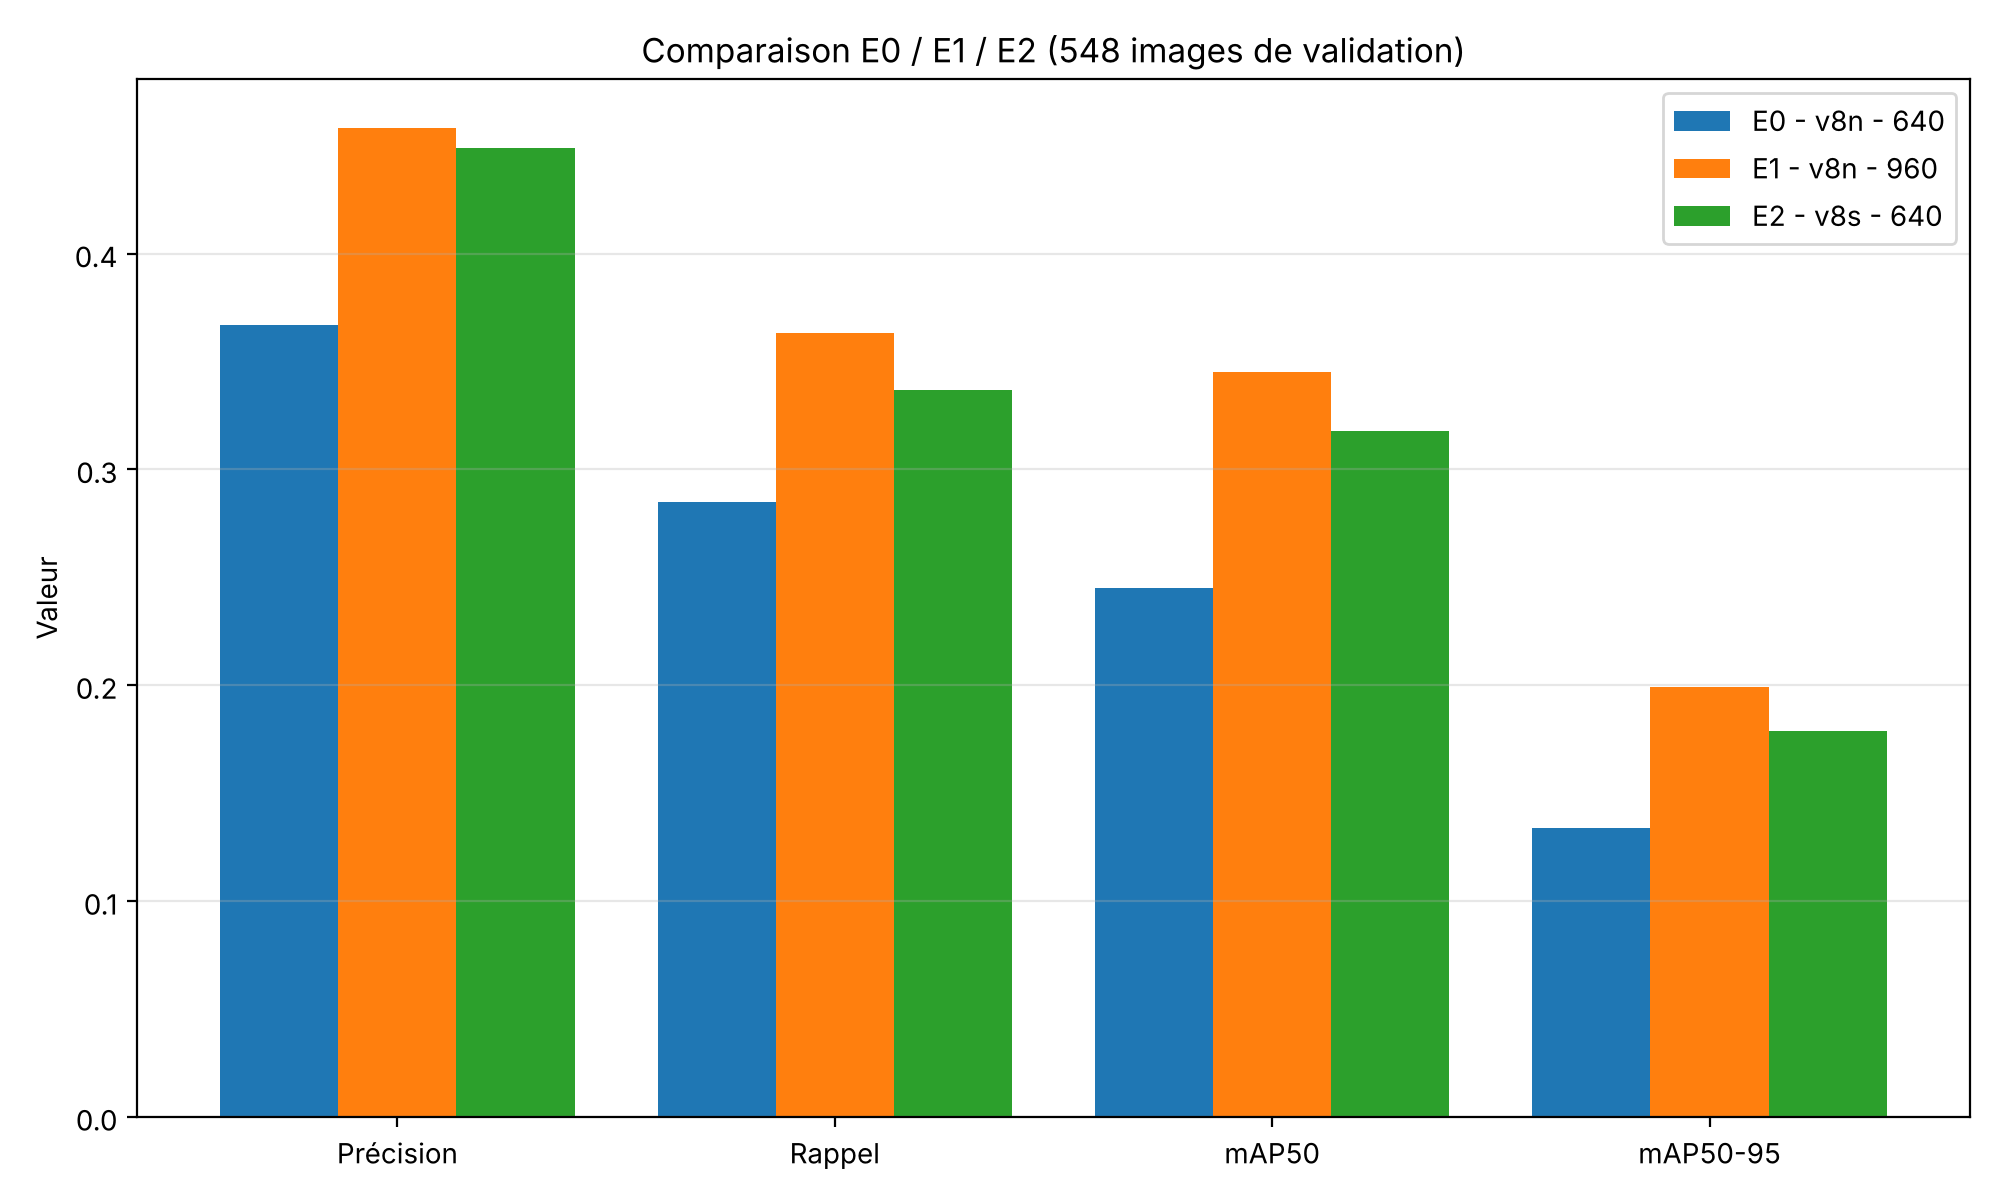
\includegraphics[width=0.8\textwidth]{indicateurs_globaux.png}
    \caption{Comparaison des indicateurs globaux.}
    \label{fig:globaux}
\end{figure}



\subsection{Résultats par classe (mAP@50)}
\begin{table}[htbp]
\centering
\small
\begin{tabular}{@{}lcccc@{}}
\toprule
Classe & E0 (n, 640) & E1 (n, 960) & E2 (s, 640) & Écart E1 $-$ E2 \\
\midrule
Pedestrian & 0,260 & 0,411 & 0,354 & +0,057 \\
People & 0,193 & 0,301 & 0,264 & +0,037 \\
Bicycle & 0,035 & 0,106 & 0,085 & +0,021 \\
Car & 0,674 & 0,772 & 0,737 & +0,035 \\
Van & 0,255 & 0,384 & 0,351 & +0,033 \\
Truck & 0,221 & 0,303 & 0,294 & +0,009 \\
Tricycle & 0,159 & 0,212 & 0,197 & +0,015 \\
Awning-tricycle & 0,063 & 0,131 & 0,107 & +0,024 \\
Bus & 0,343 & 0,441 & 0,434 & +0,007 \\
Motor & 0,246 & 0,385 & 0,354 & +0,031 \\
\bottomrule
\end{tabular}
\caption{mAP@50 par classe sur la validation.}
\label{tab:classes}
\end{table}

Pour chacune des dix classes, E1 et E2 dépassent E0, et E1 dépasse E2. La
classe \emph{car} obtient les meilleures valeurs dans les trois expériences ;
\emph{bicycle} et \emph{awning-tricycle} restent les plus difficiles.
L'avantage de la haute résolution sur le modèle plus grand est le plus
marqué pour \emph{pedestrian} (+0,057), \emph{people} (+0,037), \emph{car}
(+0,035), \emph{van} (+0,033) et \emph{motor} (+0,031), et le plus faible
pour \emph{bus} (+0,007), \emph{truck} (+0,009) et \emph{tricycle} (+0,015).
\begin{figure}[H]
    \centering
    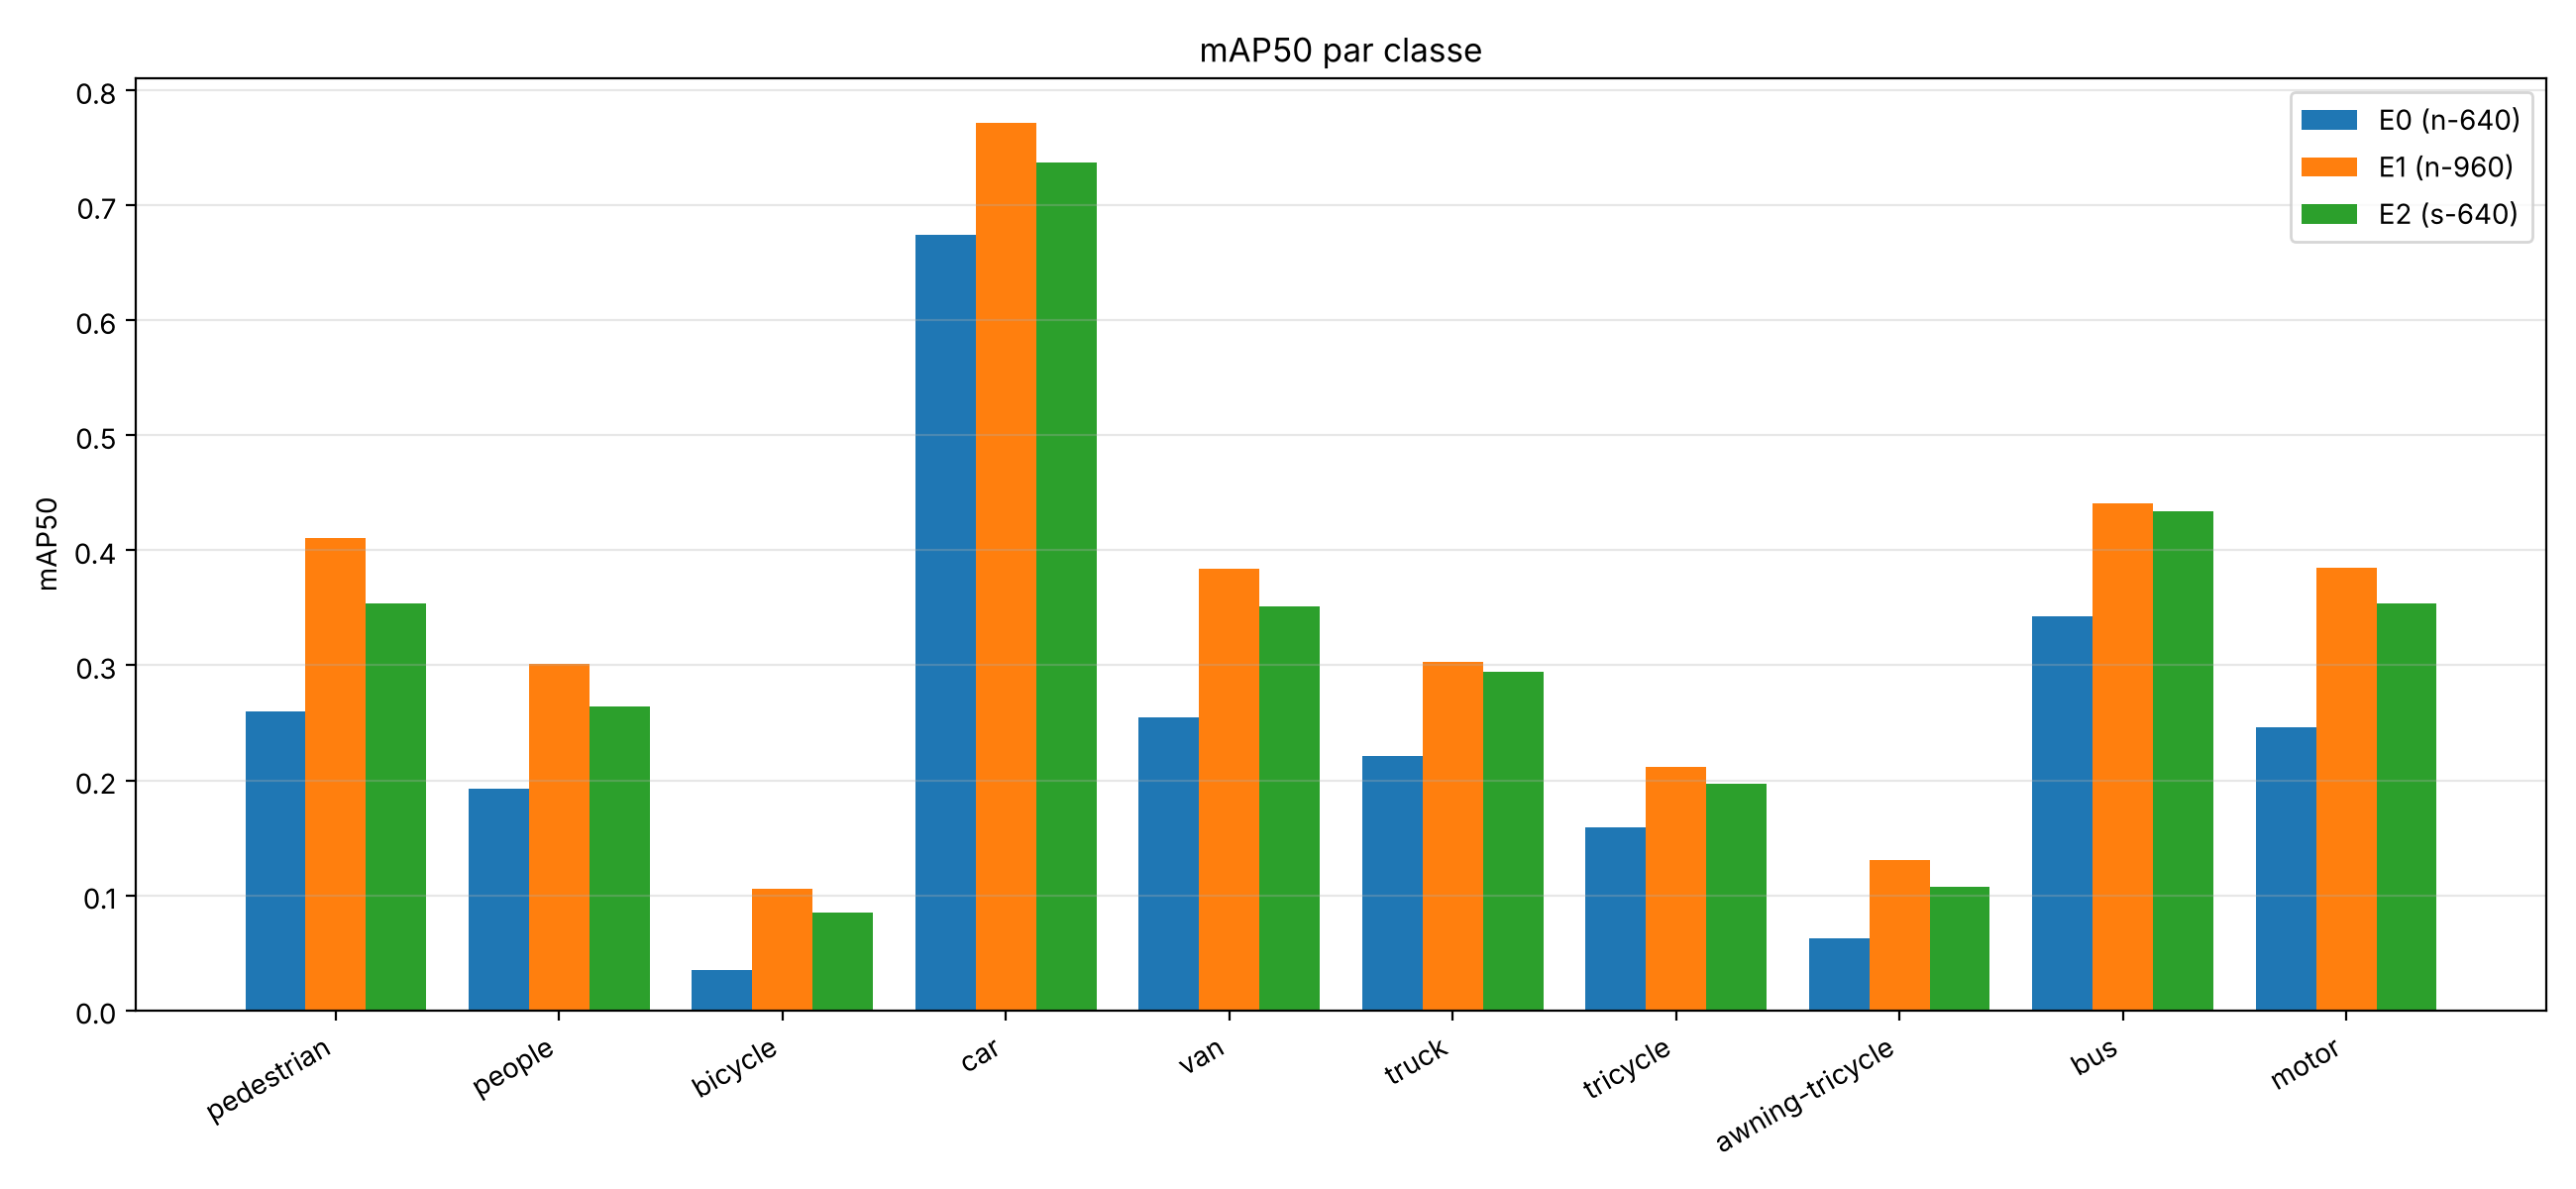
\includegraphics[width=1\textwidth]{map50_par_classe.png}
    \caption{mAP@50 par classe.}
    \label{fig:classes}
\end{figure}
% \fig[0.9]{map50_par_classe.png}{mAP@50 par classe.}{fig:classes}


\subsection{Répartition des objets par taille}
\begin{table}[htbp]
\centering
\small
\begin{tabular}{@{}lrr@{}}
\toprule
Taille & Nombre d'objets & Proportion \\
\midrule
Petits & 26\,586 & 68,59 \% \\
Moyens & 11\,105 & 28,65 \% \\
Grands & 1\,068 & 2,76 \% \\
\midrule
Total & 38\,759 & 100 \% \\
\bottomrule
\end{tabular}
\caption{Répartition des objets de validation selon leur taille.}
\label{tab:tailles}
\end{table}

Les petits objets représentent 68,59 \% des annotations de validation : ils
constituent l'enjeu principal pour un détecteur appliqué aux images de drone.

\subsection{Rappel selon la taille des objets (E0 et E1)}
\begin{table}[htbp]
\centering
\small
\begin{tabular}{@{}lccc@{}}
\toprule
Taille & E0 (640) & E1 (960) & Gain (points) \\
\midrule
Petits & 23,09 \% & 34,36 \% & +11,27 \\
Moyens & 64,77 \% & 73,65 \% & +8,88 \\
Grands & 84,08 \% & 87,64 \% & +3,56 \\
\bottomrule
\end{tabular}
\caption{Rappel par taille d'objet (IoU 0,50, confiance 0,25).}
\label{tab:rappel-taille}
\end{table}

Le gain apporté par la résolution 960 est le plus fort pour les petits objets
(+11,27 points) et diminue avec la taille des objets. Ce rappel par taille
n'a pas été calculé pour E2.


\subsection{Coût de calcul et temps}
\begin{table}[htbp]
\centering
\small
\begin{tabular}{@{}lccc@{}}
\toprule
Indicateur & E0 (n, 640) & E1 (n, 960) & E2 (s, 640) \\
\midrule
Paramètres & 3,13 M & 3,13 M & 11,13 M \\
GFLOPs à 640 (Ultralytics) & 8,6 & 8,6 & 28,5 \\
GFLOPs à 960 (estimation) & --- & $\approx$ 19 & --- \\
Temps d'entraînement (30 époques) & 24,0 min & 38,8 min & 26,8 min \\
Inférence GPU T4 (ms/image) & 3,5 & 5,4 & 4,8 \\
Inférence CPU (ms/image) & 124,2 & 295,4 & non mesuré \\
\bottomrule
\end{tabular}
\caption{Coût de calcul et temps.}
\label{tab:cout}
\end{table}

Les GFLOPs d'E1 à 960 sont une estimation ($8{,}6 \times (960/640)^2
\approx 19$), non une mesure. Sur CPU, E1 est environ 2,38 fois plus lent
qu'E0 (prétraitement 3,2 contre 8,5 ms, post-traitement 20,6 contre 35,2 ms
par image), ce qui est cohérent avec l'augmentation du nombre de pixels
(facteur 2,25). Les temps GPU proviennent d'une seule passe de validation ;
les temps de prétraitement et de post-traitement varient d'une passe à
l'autre, de sorte que des écarts de l'ordre de la milliseconde ne sont pas
significatifs. Les durées d'entraînement proviennent de sessions différentes
et sont indicatives.
\begin{figure}[H]
    \centering
    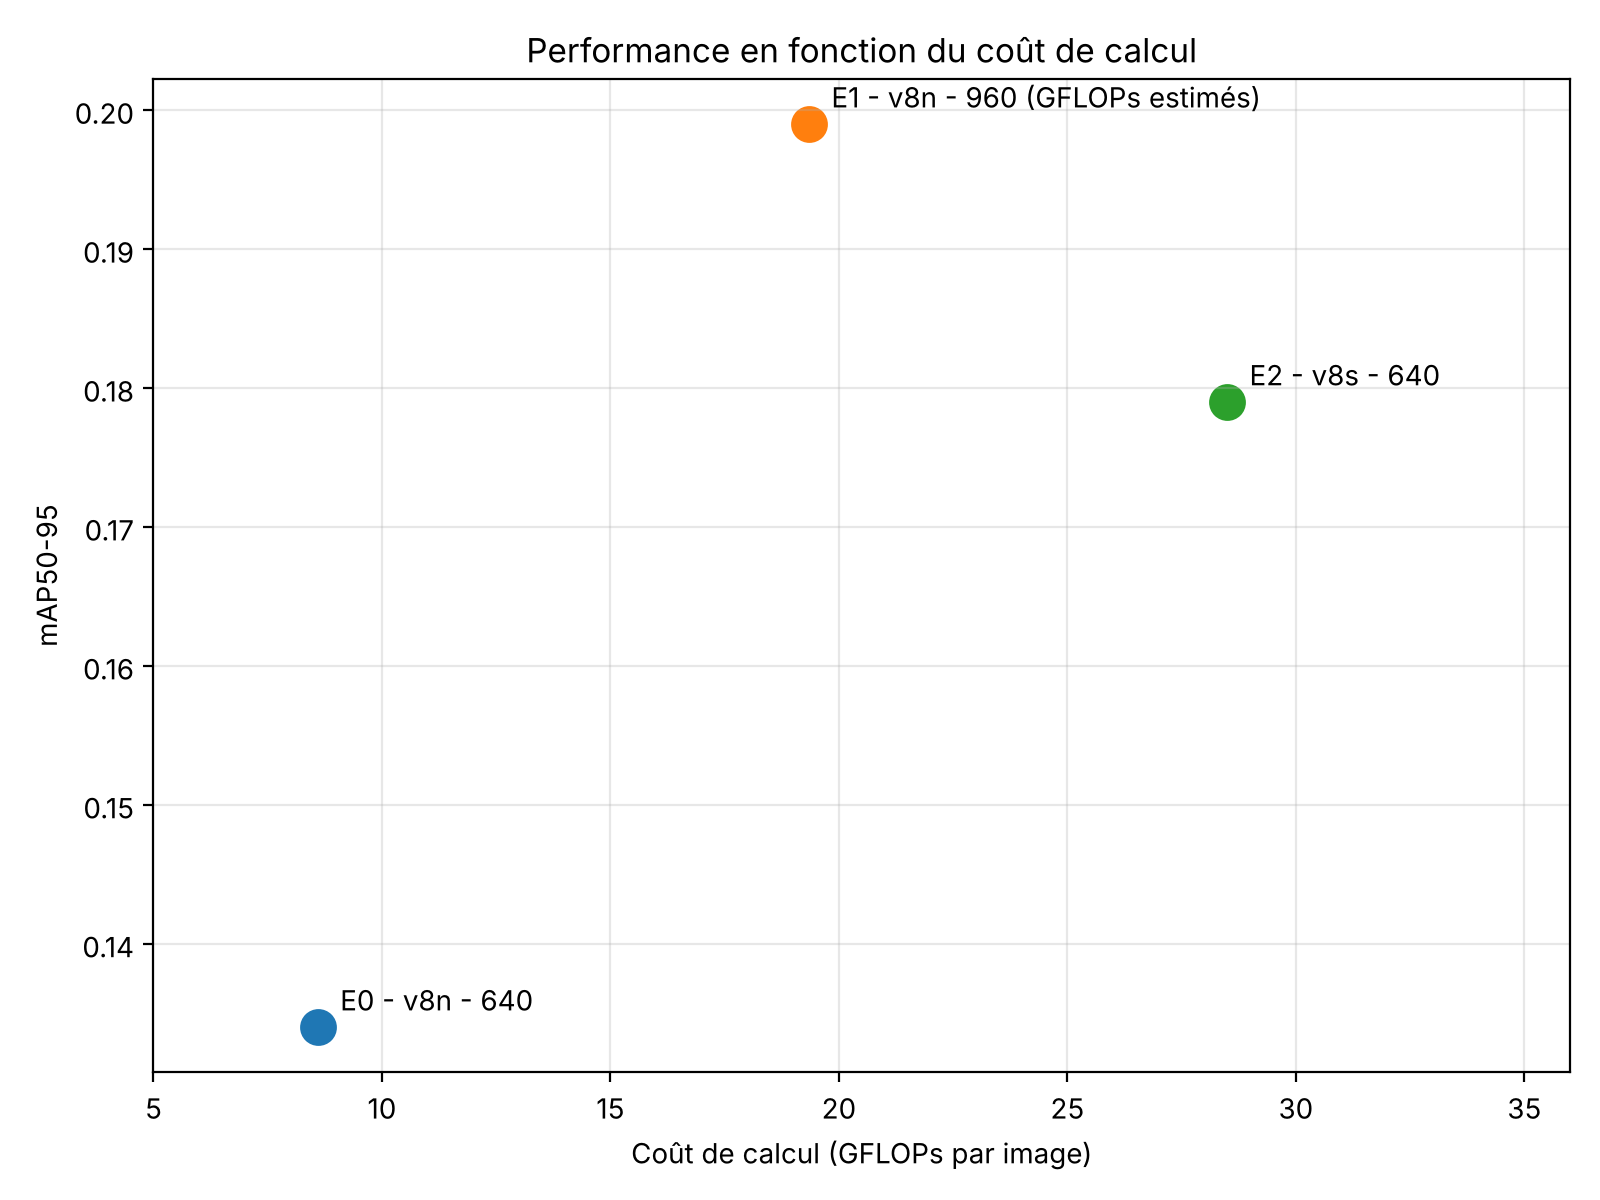
\includegraphics[width=0.7\textwidth]{compromis_precision_calcul.png}
    \caption{Performance et coût de calcul.}
    \label{fig:compromis}
\end{figure}
% \fig[0.85]{compromis_precision_calcul.png}{Performance et coût de calcul.}{fig:compromis}



% #########DISCUSSION###############


\section{Discussion}
\label{sec:discussion}

\textbf{Effet de la taille du modèle.} À résolution égale, passer de YOLOv8n
à YOLOv8s améliore nettement les résultats (mAP@50 : 0,245 à 0,318, soit
+29,8 \%), au prix d'un modèle environ 3,5 fois plus grand et d'un coût de
calcul environ 3,3 fois plus élevé en GFLOPs.

\textbf{Effet de la résolution.} À modèle égal, passer de 640 à 960 améliore
davantage les résultats (mAP@50 : 0,245 à 0,345, soit +40,8 \%), sans
augmenter le nombre de paramètres. Le résultat le plus notable est qu'un
petit modèle à haute résolution (E1) dépasse un modèle plus grand à
résolution standard (E2) sur les quatre indicateurs globaux, pour un coût de
calcul estimé plus faible (environ 19 contre 28,5 GFLOPs).

\textbf{Rôle des petits objets.} Les petits objets représentent plus des
deux tiers des annotations. Le rappel par taille (E0 et E1) montre que le
gain de la résolution est le plus fort pour eux (+11,27 points contre +3,56
pour les grands objets). Par classe, l'avantage d'E1 sur E2 est le plus
marqué pour \emph{pedestrian}, \emph{people} et \emph{motor}, classes dont
les instances sont souvent petites, et faible pour \emph{bus} et
\emph{truck}, souvent plus grands. Cette tendance est cohérente avec
l'explication selon laquelle une résolution plus élevée conserve des détails
spatiaux utiles aux petits objets. Elle n'est cependant pas uniforme
(l'écart est aussi notable pour \emph{car} et \emph{van}) et, sans rappel ni
mAP par taille calculé pour E2, elle reste une interprétation plausible
plutôt qu'une démonstration.

\textbf{Compromis.} La résolution 960 augmente le temps d'inférence
(environ 2,4 fois sur CPU) et le temps d'entraînement (38,8 contre 24,0
minutes). Pour une application temps réel sur matériel limité, la
résolution 640 peut rester pertinente ; si la détection des petits objets
est prioritaire et qu'un traitement plus long est acceptable, E1 offre le
meilleur rapport entre performance et coût dans cette étude.

\section{Limites de l'étude}
\label{sec:limites}
\begin{itemize}
  \item Entraînement sur un sous-ensemble de 2\,000 images (sur 6\,471
        disponibles) et seulement 30 époques.
  \item Une seule graine aléatoire (0) : aucune répétition ne permet
        d'estimer la variabilité. Les écarts de quelques millièmes (par
        exemple les différences de précision entre E1 et E2) ne sont pas
        significatifs.
  \item Les classes rares (\emph{bicycle}, \emph{awning-tricycle},
        \emph{bus}) comptent peu d'instances ; leurs valeurs sont moins
        fiables.
  \item Le rappel par taille est un indicateur personnalisé (confiance
        0,25, IoU 0,50), calculé pour E0 et E1 uniquement, et non un mAP
        par taille officiel.
  \item Les temps d'inférence GPU proviennent d'une seule passe et sont
        bruités ; les temps CPU n'existent que pour E0 et E1. Les temps
        d'entraînement viennent de sessions Colab différentes.
  \item Le plan expérimental est incomplet : la combinaison YOLOv8s à 960
        pixels (E3) n'a pas été réalisée, ce qui empêche de savoir si les
        gains de la taille du modèle et de la résolution s'additionnent.
  \item Le jeu de test n'a pas été utilisé : les conclusions reposent sur
        la validation.
\end{itemize}

\section{Conclusion et perspectives}
\label{sec:conclusion}
Ce projet a comparé trois configurations de YOLOv8 sur VisDrone2019-DET avec
les mêmes données d'entraînement et d'évaluation. Passer de 640 à 960 pixels
(E1) et passer de YOLOv8n à YOLOv8s (E2) améliorent tous deux les résultats
par rapport à la référence E0. La résolution a l'effet le plus important :
E1 obtient un mAP@50 de 0,345 et un mAP@50-95 de 0,199, contre 0,318 et 0,179
pour E2, avec un modèle environ 3,5 fois plus léger. L'analyse par taille
indique que le bénéfice de la résolution est le plus fort pour les petits
objets, qui forment 68,59 \% des objets de validation. En contrepartie, la
haute résolution augmente le temps de calcul.

Pour approfondir ce travail, il serait pertinent de réaliser E3 (YOLOv8s à
960), de calculer le rappel et le mAP par taille pour tous les modèles,
d'entraîner sur l'ensemble des images disponibles avec plus d'époques, de
répéter les expériences avec plusieurs graines, d'évaluer les meilleurs
modèles sur le jeu de test et de comparer avec des stratégies dédiées aux
petits objets.




%#################REFERENCE ET BIBLIOGRAPHY
%##########################ARTICLE +  SOURCE


\begin{thebibliography}{99}

\bibitem[Redmon et~al.(2016)]{redmon2016yolo}
J.~Redmon, S.~Divvala, R.~Girshick et A.~Farhadi.
\newblock You Only Look Once: Unified, Real-Time Object Detection.
\newblock In \emph{IEEE Conference on Computer Vision and Pattern Recognition (CVPR)}, 2016, pp.~779--788.

\bibitem[Girshick et~al.(2014)]{girshick2014rich}
R.~Girshick, J.~Donahue, T.~Darrell et J.~Malik.
\newblock Rich Feature Hierarchies for Accurate Object Detection and Semantic Segmentation.
\newblock In \emph{CVPR}, 2014, pp.~580--587.

\bibitem[Girshick(2015)]{girshick2015fast}
R.~Girshick.
\newblock Fast R-CNN.
\newblock In \emph{IEEE International Conference on Computer Vision (ICCV)}, 2015.

\bibitem[Ren et~al.(2015)]{ren2015faster}
S.~Ren, K.~He, R.~Girshick et J.~Sun.
\newblock Faster R-CNN: Towards Real-Time Object Detection with Region Proposal Networks.
\newblock In \emph{Advances in Neural Information Processing Systems (NeurIPS)}, 2015.

\bibitem[Zou et~al.(2019)]{zou2019object}
Z.~Zou, K.~Chen, Z.~Shi, Y.~Guo et J.~Ye.
\newblock Object Detection in 20 Years: A Survey.
\newblock \emph{arXiv:1905.05055}, 2019.

\bibitem[Jocher et~al.(2023)]{jocher2023ultralytics}
G.~Jocher, A.~Chaurasia et J.~Qiu.
\newblock Ultralytics YOLOv8, 2023.
\newblock \url{https://github.com/ultralytics/ultralytics} --- documentation : \url{https://docs.ultralytics.com/}.

\bibitem[Zhu et~al.(2020)]{zhu2020visdrone}
P.~Zhu, L.~Wen, D.~Du, X.~Bian, H.~Fan, Q.~Hu et H.~Ling.
\newblock Detection and Tracking Meet Drones Challenge.
\newblock \emph{arXiv:2001.06303}, 2020. Jeu de données : \url{https://github.com/VisDrone/VisDrone-Dataset}.

\bibitem[Du et~al.(2019)]{du2019visdrone}
D.~Du et~al.
\newblock VisDrone-DET2019: The Vision Meets Drone Object Detection in Image Challenge Results.
\newblock In \emph{IEEE/CVF International Conference on Computer Vision Workshops (ICCVW)}, 2019.

\bibitem[Lin et~al.(2014)]{lin2014coco}
T.-Y. Lin, M.~Maire, S.~Belongie, J.~Hays, P.~Perona, D.~Ramanan, P.~Doll{\'a}r et C.~L. Zitnick.
\newblock Microsoft COCO: Common Objects in Context.
\newblock In \emph{European Conference on Computer Vision (ECCV)}, 2014, pp.~740--755.

\end{thebibliography}
\end{document}